\documentclass[border=1mm]{standalone}

\usepackage{import}
\subimport{../../../}{preamble.tex}

\usepackage{tikz}
\usetikzlibrary{calc}
\usepackage{pgfplots}

\begin{document}

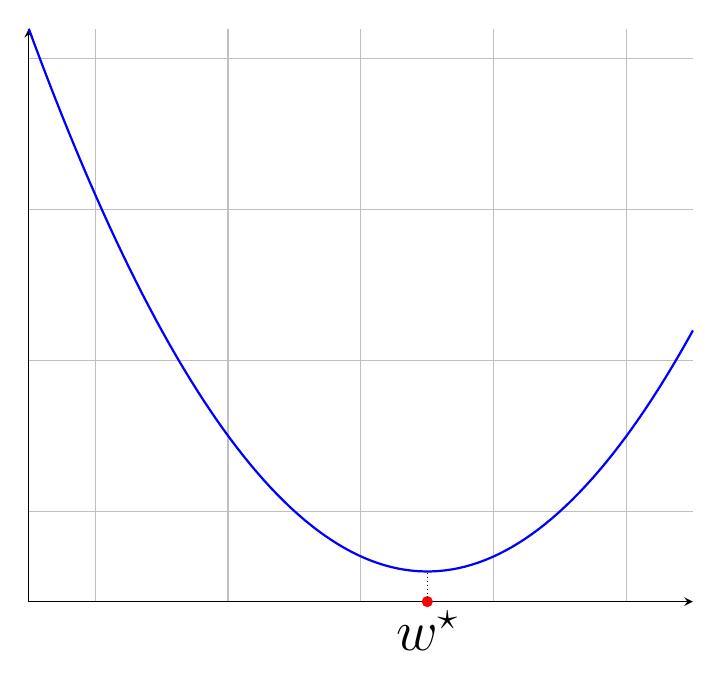
\begin{tikzpicture}
  \begin{axis}[
    scale only axis,
    grid=major,
    axis lines=left,
    inner axis line style={=>},
    ticks=none,
    clip=false,
    ymin=-6,
%    title{$\norm{Y - X w}^2_2$}
    ]
    \addplot[color=blue,thick,samples=100] {(x-1)^2-4};
    \node[circle, fill=red, inner sep=0.5mm] (wstar) at (axis cs:1,-6) {};
    \node[below] at (axis cs:1,-6) {\huge $w^\star$};
    \draw[densely dotted] (axis cs:1,-6) -- (axis cs:1,-4);
    
  \end{axis}
\end{tikzpicture}

\end{document}

%%% Local Variables:
%%% mode: latex
%%% TeX-master: t
%%% End:
